\subsection{Bildverarbeitung}

\subsubsection{Versuchsbeschreibung}
Für die Erkennung des Korbes wurde ein Testprogramm in Java geschrieben. Es wurden Fotos des Korbes aus verschiedenen Blickwinkeln und auf unterschiedlichem Hintergrund angefertigt. Mittels dem OpenCV-Framework, welches frei erhältlich ist, wurden verschiedene Algorithmen auf das Bild angewandt um den Korb vom Hintergrund abzugrenzen.

\cite{img:info}

\subsubsection{Vorbereitung}
Zu Testzwecken werden verschiedene Fotos von einem schwarzen Korb angefertigt. 
Es gibt zwei unterschiedliche Hintergrundszenarien. Bei jedem Hintergrund wird der 
Korb an 3 verschiedenen Stellen platziert.

\begin{figure}[h!]
    \centering
    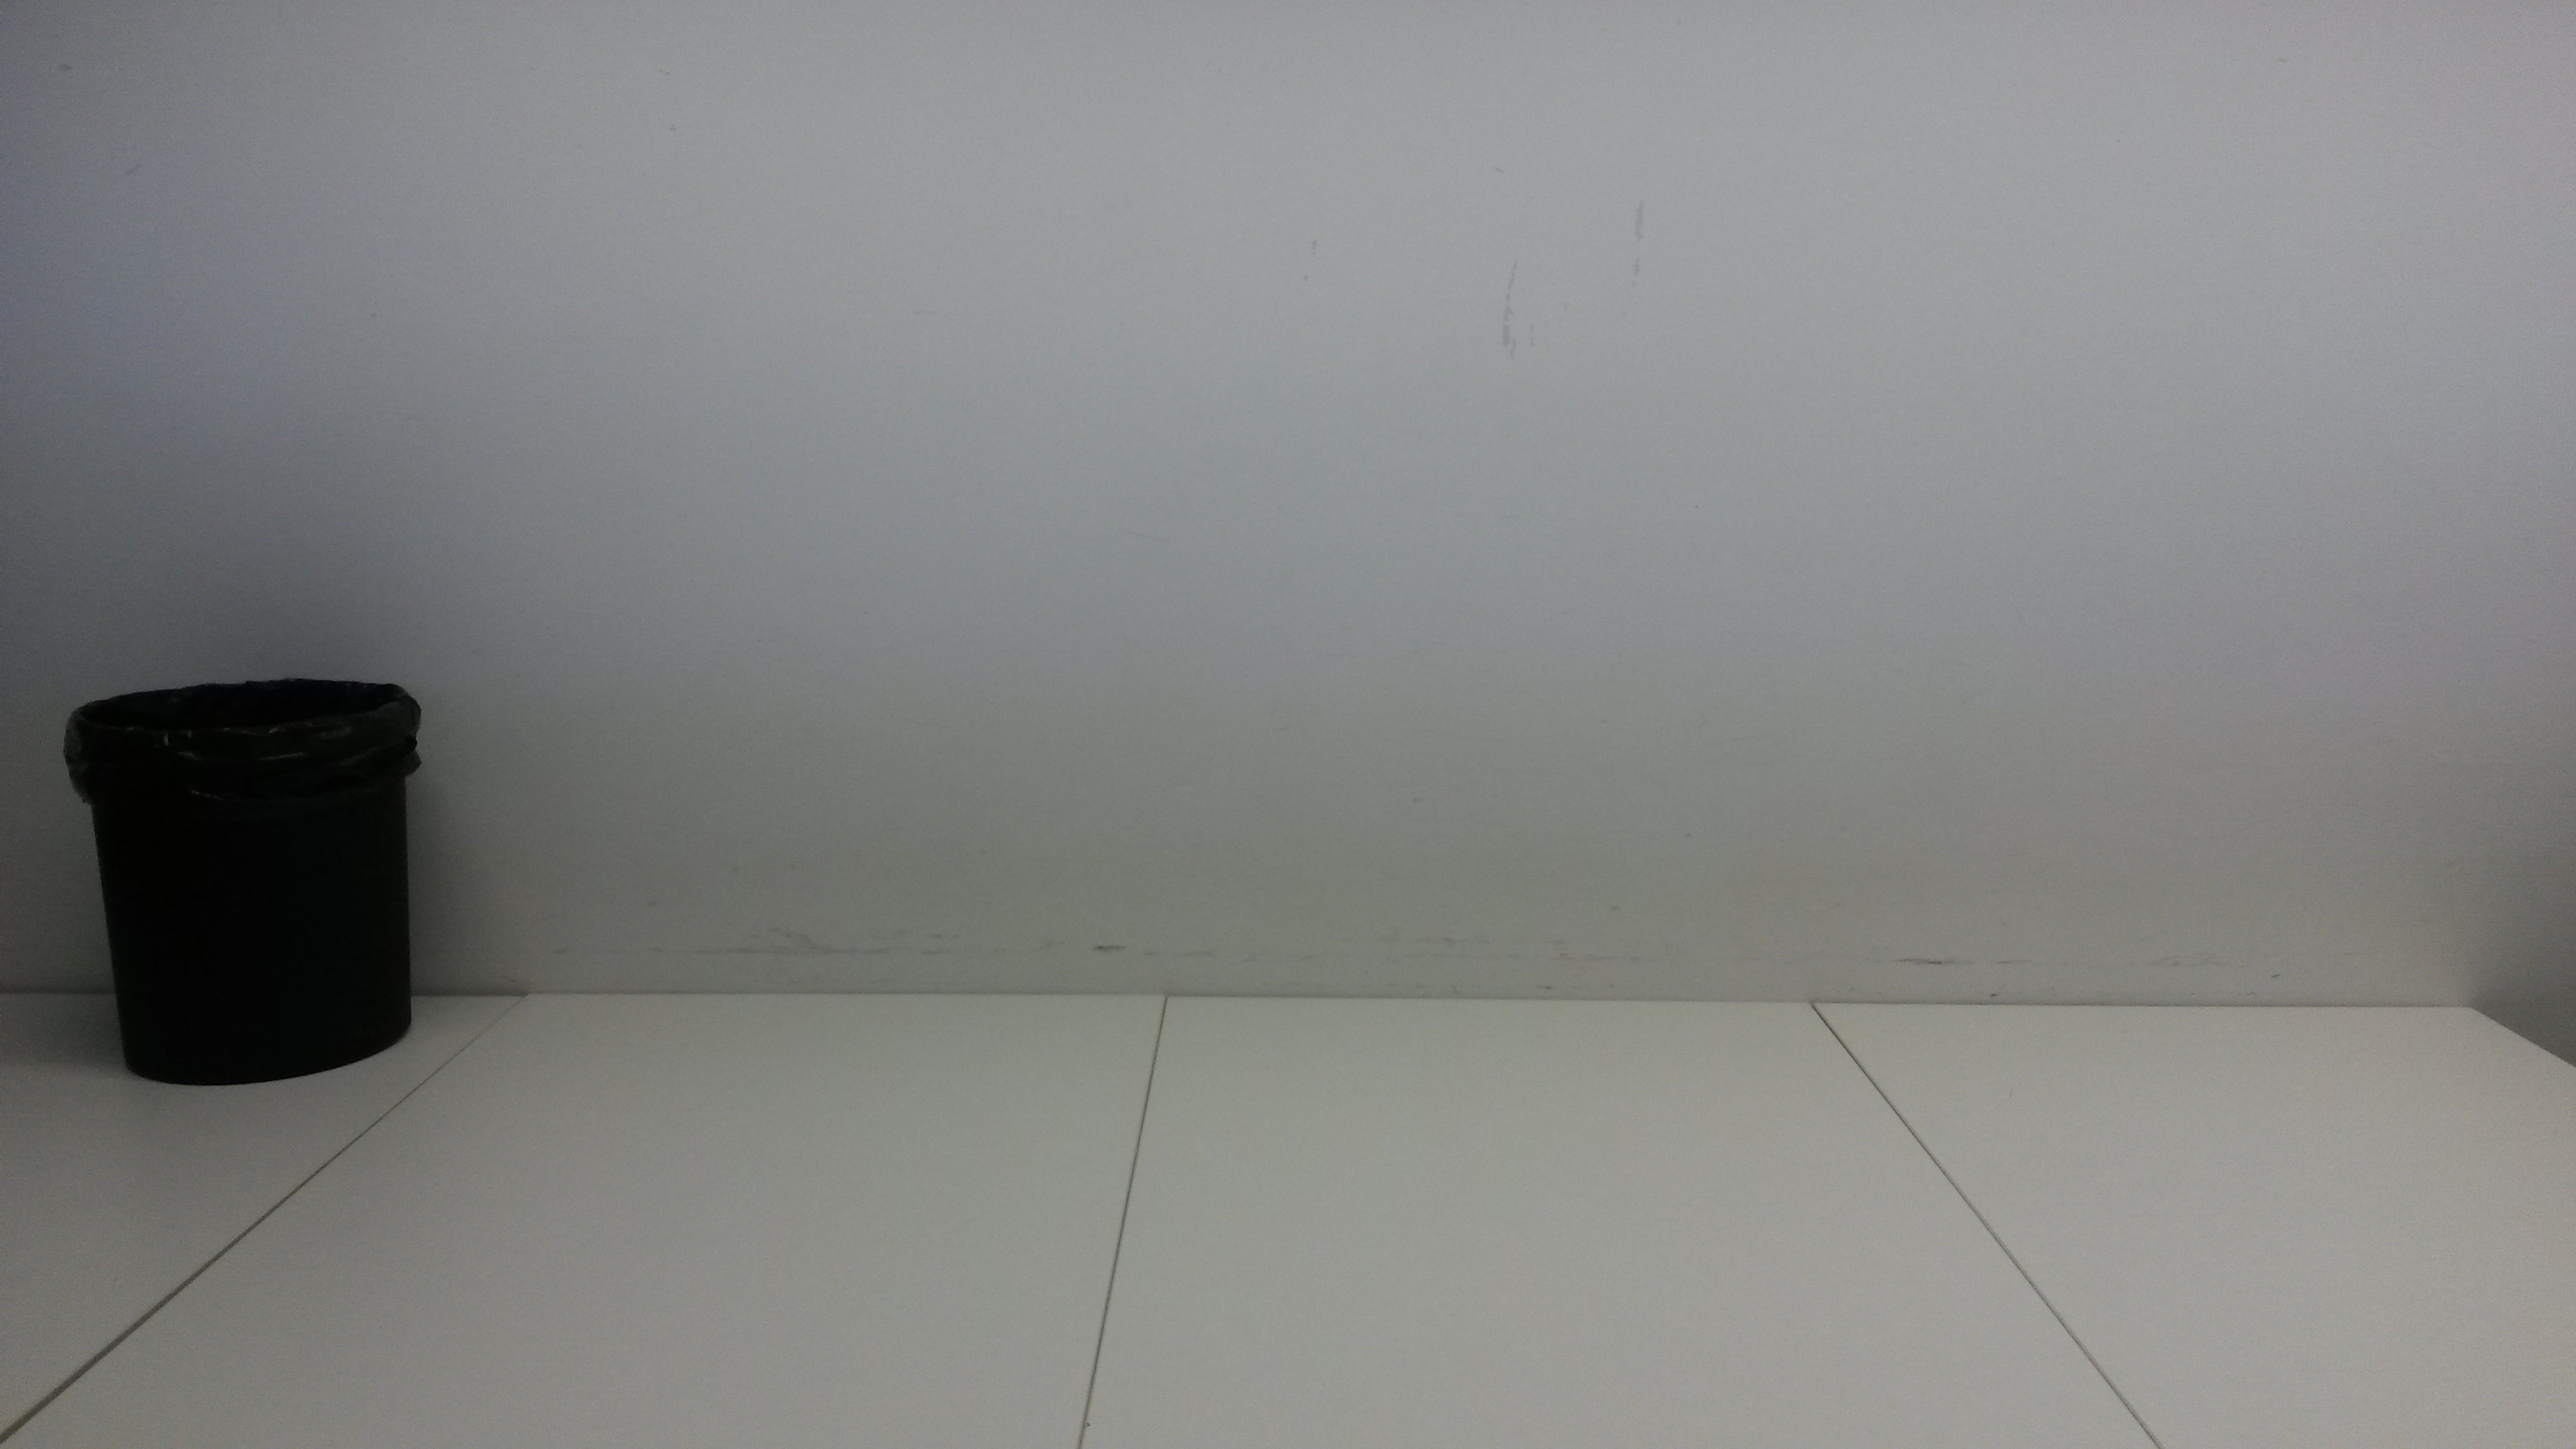
\includegraphics[width=0.5\textwidth]{fig/korb4.jpg}
    \caption{Beispielbild mit Hintergrund einfarbig}
    \label{fig:Korb_HEinfarbig}
\end{figure}

\begin{figure}[h!]
    \centering
    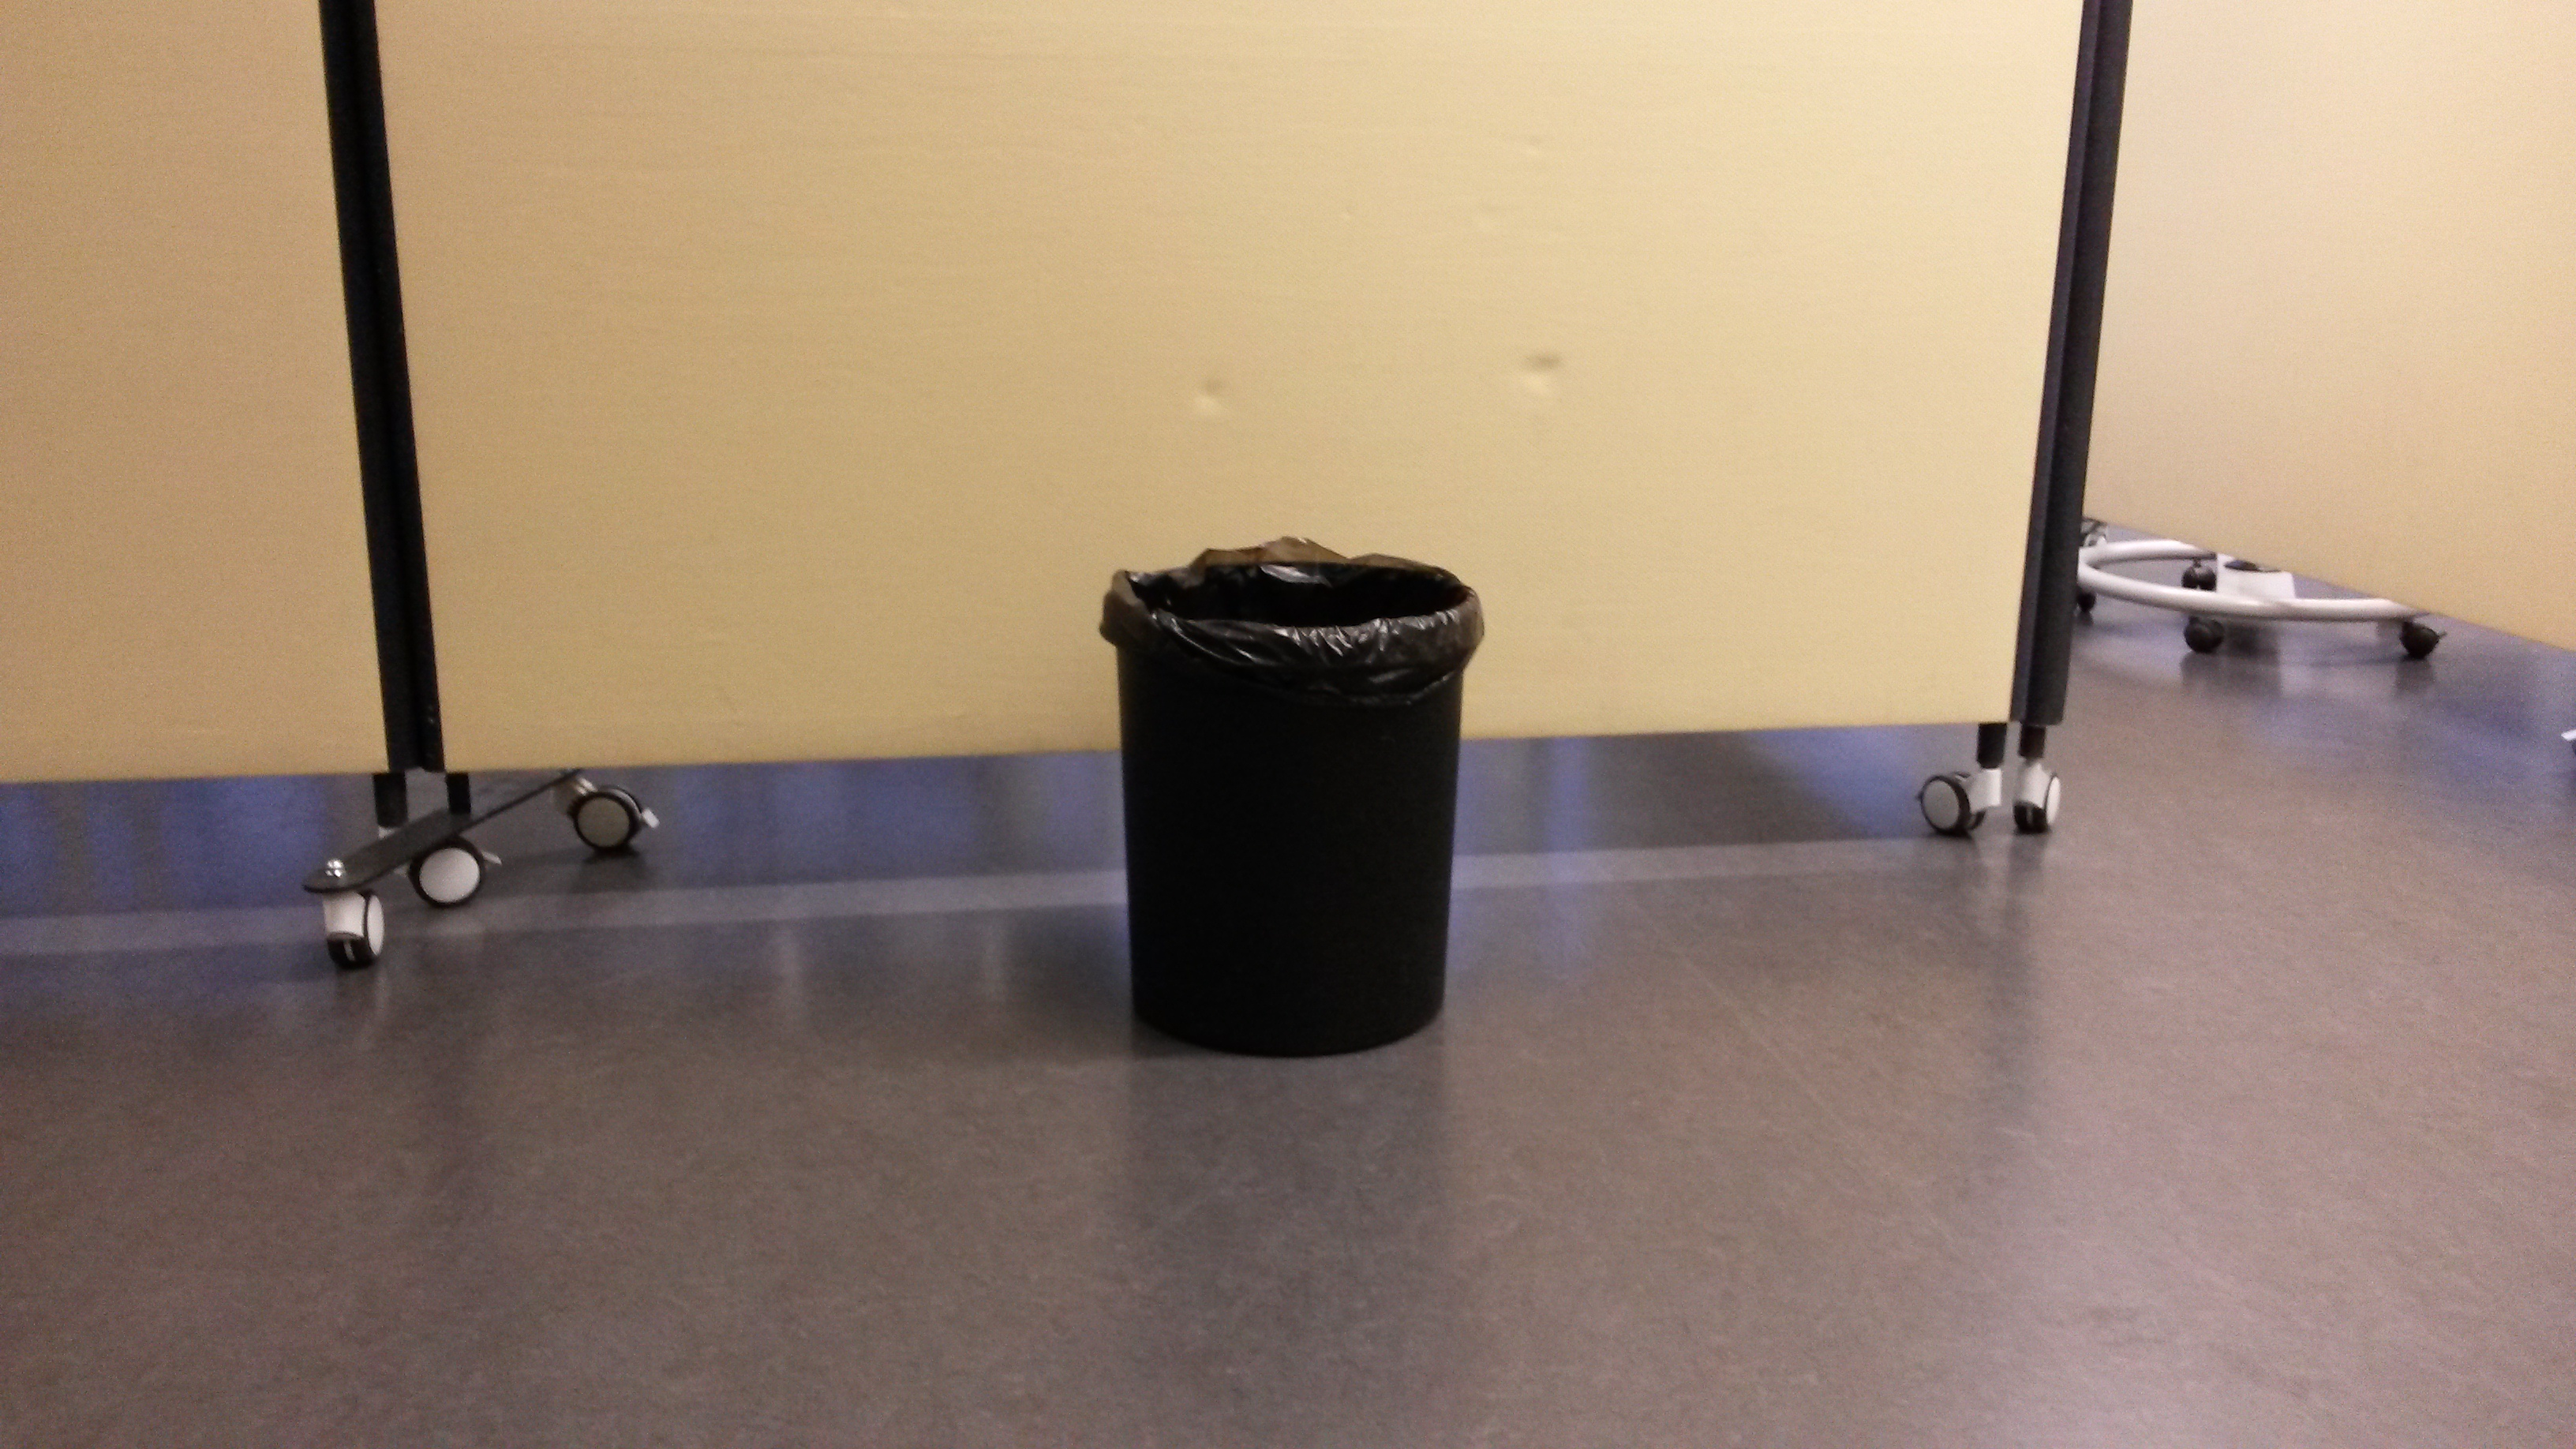
\includegraphics[width=0.5\textwidth]{fig/korb1.jpg}
    \caption{Beispielbild mit Hintergrund enthält schwarz}
    \label{fig:Korb_HSchwarz}
\end{figure}

\noindent Abbildung \ref{fig:Korb_HSchwarz} zeigt einen Hintergrund bei dem zusätzlich 
noch schwarze Farbe vorkommt. Dies erhöht den Schwierigkeitsgrad  den Korb zu 
erkennen, da der Suchvorgang falsche Informationen verwerten kann. Bei 
Abbildung \ref{fig:Korb_HEinfarbig} ist der Hintergrund möglichst einfarbig 
gehalten um ein gegensätzliches Szenario zu Abbildung \ref{fig:Korb_HSchwarz} 
zu erhalten.

\subsubsection{Erkennung}
Im folgenden Abschnitt wird beschrieben, wie das Vorgehen zur Erkennung des Korbes 
gewählt wurde. Ebenfalls werden die Ergebnisse präsentiert.\\
%
Als erstes wird eines der Beispielbilder geladen.\\
%
Es folgen diese Schritte:\\
%
\begin{itemize}
    \item Das Bild wird geladen und in ein HSV-Bild umgewandelt
    \begin{itemize}
        \item HSV steht für einen Farbwertebereich der mit Hue, Saturation, 
            Value beschrieben wird.
        \item Im Folgenden ein Bild des HSV-Farbbereichs:\\
        \begin{figure}[h!]
            \centering
            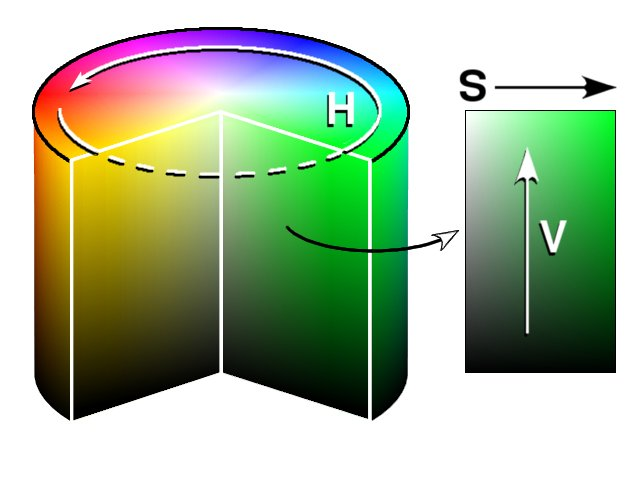
\includegraphics[width=0.5\textwidth]{fig/HSV_cylinder.jpg}
            \caption[HSV-Farbspektrum]{HSV-Farbspektrum \cite{wiki:gimp2_farbmodelle}}
            \label{fig:HSV-Farbspektrum}
        \end{figure}
    \end{itemize}
    \item Es folgt eine HSV-Filterung. Dafür sind beim erstellten Programm drei 
        Slider angebracht, um mit den Werten zu experimentieren und die 
        optimalen Ergebnisse zu erzielen, beim Erzeugen eines Schwarz-Weiss Bildes.
    \begin{itemize}
        \item Die zwei Slider für Hue und Saturation sind auf den Minimumwert 0 
            und Maximalwert 256 eingestellt. Diese können so belassen werden.
        \item Der dritte Slider steht für den Value, mit welchem die dunklen Werte 
            gefiltert werden. Hier wird mit einer Grundeinstellung von Minimum 
            null und Maximal 15 gearbeitet.
        \begin{itemize}
            \item Zum Experimentieren kann der Slider verschoben werden und 
                der Filter erneut angewendet werden.
        \end{itemize}
    \end{itemize}
    \item Nach der Filterung ist das Bild noch von „Farbrauschen“ erfüllt. 
        Dieses Rauschen wird mit dem „Eroden“ herausgefiltert.
    \begin{itemize}
        \item Für das Erodieren wird mit einem 5$\times$5 Pixel grossem Filter gearbeitet. 
            Alles was diesem Wert entspricht wird von Weiss in Schwarz 
            umgewandelt.
        \item So werden kleine ungewollte weisse Pixel aus dem Bild entfernt.
        \item Dieser Vorgang wird zwei Mal auf das Bild angewendet.
    \end{itemize}
    \item Nach dem Erodieren muss noch ein „Dilate“ ausgeführt werden.
    \begin{itemize}
        \item Damit wird ungewolltes Entfernen rückgängig gemacht 
            indem die Pixelflächen wieder vergrössert werden.
        \item Hier wird mit einem Wert von 15$\times$15 Pixeln gearbeitet.
        \item Das „Dilate“-Element wird zweimal auf das Bild angewendet.
    \end{itemize}
    \item Nach diesen Massnahmen sollte nur noch der Korb als weisse Fläche 
        auf dem Bild zu sehen sein und der Rest ist schwarz.
\end{itemize}

Ergebnis für die Abbildung \ref{fig:Korb_HEinfarbig} nach dem Anwenden der 
Filter sieht folgendermassen aus:

\begin{figure}[h!]
    \centering
    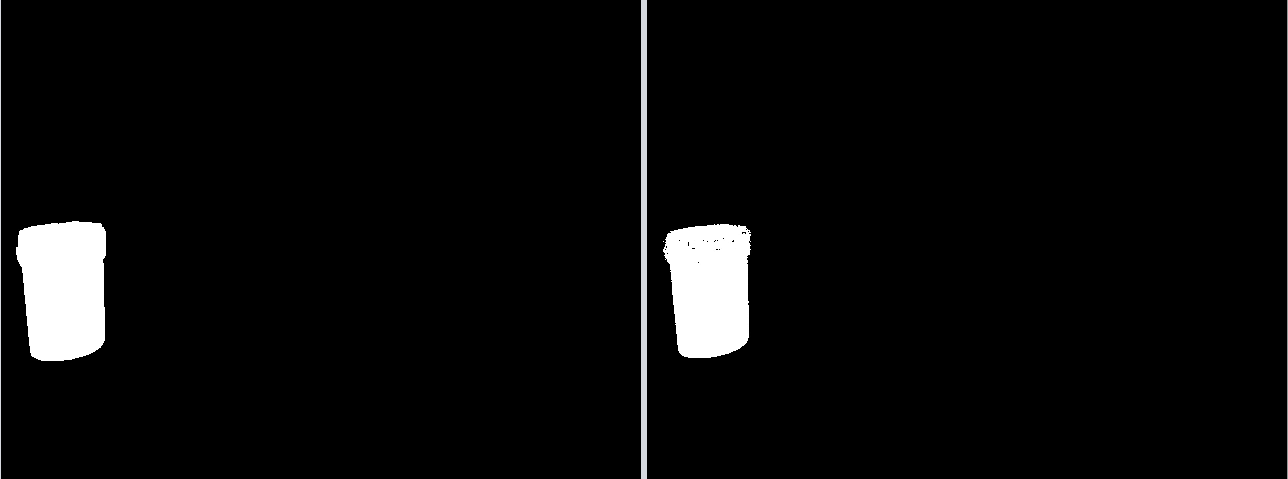
\includegraphics[width=0.7\textwidth]{fig/Korberkennung1.png}
    \caption{Links nach Erode und Dilate - Rechts nur mit HSV Filterung}
    \label{fig:Korb_Erkennung}
\end{figure}

\subsubsection{Testprogramm}
Anbei sieht man ein Screenshot des Testprogramms:
\begin{figure}[h!]
    \centering
    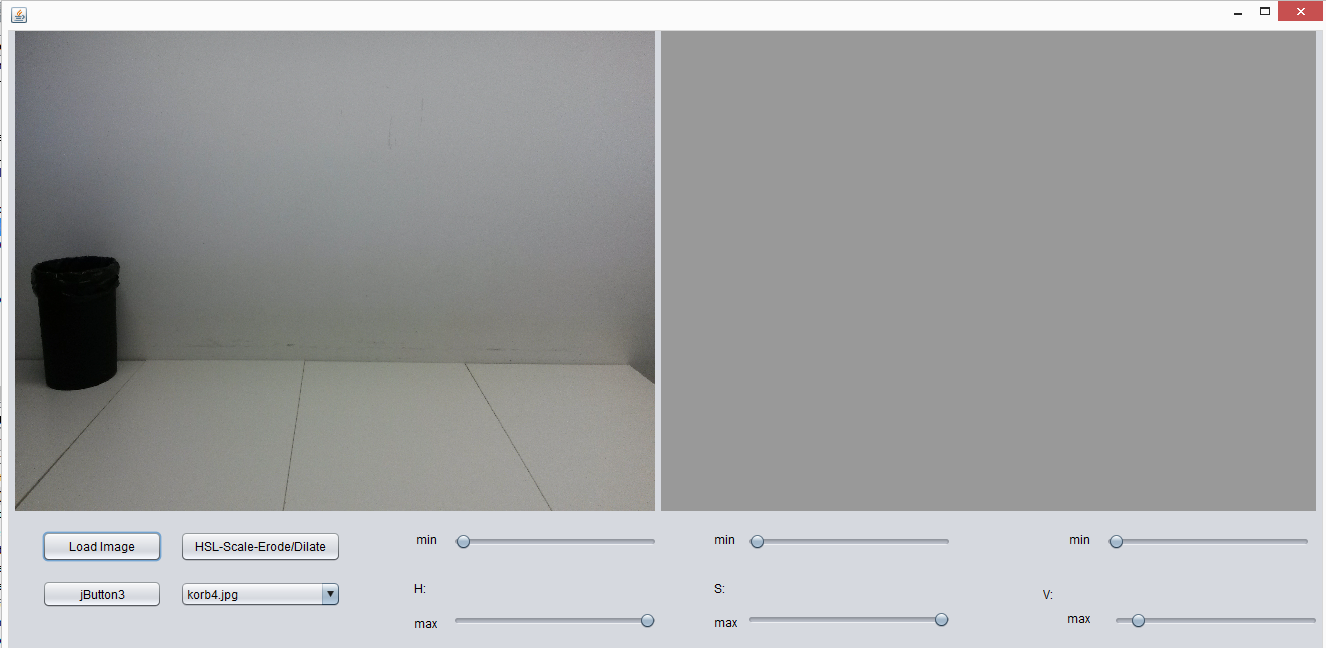
\includegraphics[width=0.7\textwidth]{fig/Testprogramm.png}
    \caption{Screenshot Testprogramm}
    \label{fig:Korb_Testprogramm}
\end{figure}

\noindent Abbildung \ref{fig:Korb_Testprogramm} zeigt die Einstellungsmöglichkeiten des 
Testprogramms. Es können mittels Slider die Werte für Hue, Saturation und 
Value angepasst werden. Nach einem Klick auf den Button wird der Filter mit 
den angegebenen HSV-Werten ausgeführt und in den zwei Bereichen dargestellt. 
Rechts nur der HSV-Filter und links mit dem ausgeführten "{}Erode"{} und "{}Dilate"{} (wie in Abbildung 
\ref{fig:Korb_Erkennung} ersichtlich ist). \\
Über den Load Image Button können verschiedene Bilder geladen werden, welche 
im Dropdownmenu zur Verfügung stehen.
